The Multi-Aquifer Well (MAW) Package calculates the saturated conductance between a multi-aquifer well and a connected groundwater flow (GWF) cell from the well and aquifer properties and the length of the well screen within the cell \citep[\S 7]{modflow6gwf}. By default, every multi-aquifer well connection is assumed to be vertical, so the in-cell screen length is taken to be the vertical screen thickness, $\mli{TOPSCRN}_n - \mli{BOTSCRN}_n$. For a non-vertical (slanted or horizontal) well, however, the actual length of screen within a cell is longer than its vertical extent, and using the vertical thickness underestimates the saturated conductance.

When the \texttt{NON\_VERTICAL\_WELLS} option is specified, the in-cell screen length of connections listed in the \texttt{ANGLEDATA} block is calculated from the screen top, screen bottom, well radius, and a tilt angle, and the saturated conductance is scaled accordingly. The tilt-angle convention follows the Multi-Node Well (MNW2) Package for \mf~\citep{konikow2009}. The full directional (ellipsoidal) conductance formulation of \cite{konikow2009} is not implemented; instead, a length correction is applied to the conductance calculated by the existing MAW conductance equations, as described below.

\subsection{Multi-Aquifer Well Conductance Equations}

The saturated conductance $C^0_{\mli{MAW},n}$ between a multi-aquifer well and connected GWF cell $n$ is calculated using one of five conductance equations selected with the \texttt{CONDEQN} keyword \citep[\S 7]{modflow6gwf}. The equations use the well radius $r_w$ (\texttt{RADIUS}), the skin (filter pack) radius $r_s$ (\texttt{RADIUS\_SKIN}), the skin hydraulic conductivity $K_s$ (\texttt{HK\_SKIN}), the geometric-mean horizontal hydraulic conductivity of the connected cell $K_h = \sqrt{K_{11} K_{22}}$, the saturated thickness of the well screen in the cell $b$, and an effective external radius $r_0$. The effective radius is

\begin{equation}
	\label{eqn:mawnv-r0}
	r_0 = \sqrt{\frac{A_n}{8 \pi}},
\end{equation}

\noindent where $A_n$ is the horizontal area of cell $n$; for a square cell $r_0 \approx 0.2 \, \Delta x$, consistent with \cite{peaceman1983}. For the \texttt{THIEM}, \texttt{SKIN}, and \texttt{CUMULATIVE} equations the screen spans the full cell, so $b$ is the cell saturated thickness; for the \texttt{MEAN} equation $b$ is the specified screen interval ($\mli{TOPSCRN}_n - \mli{BOTSCRN}_n$). The length correction described in this chapter replaces $b$ with the in-cell screen length $L_w$ for non-vertical connections.

The \texttt{SPECIFIED} equation uses a saturated conductance, $C_{\mli{spec},n}$, supplied directly by the user. The \texttt{THIEM} equation uses the Thiem equation for radial flow to the well,

\begin{equation}
	\label{eqn:mawnv-thiem}
	C^0_{\mli{MAW},n} = \frac{2 \pi K_h b}{\ln(r_0 / r_w)} .
\end{equation}

\noindent The \texttt{SKIN} equation accounts for a skin (filter pack) of hydraulic conductivity $K_s$ and radius $r_s$,

\begin{equation}
	\label{eqn:mawnv-skin}
	C^0_{\mli{MAW},n} = \frac{2 \pi K_h b}{\left( \frac{K_h}{K_s} - 1 \right) \ln(r_s / r_w)} ,
\end{equation}

\noindent and the program terminates with an error if the transmissivity contrast $K_h / K_s$ is not greater than one. The \texttt{CUMULATIVE} equation combines the Thiem and skin terms (and is equivalent to the SKIN loss type of the MNW2 Package),

\begin{equation}
	\label{eqn:mawnv-cumulative}
	C^0_{\mli{MAW},n} = \frac{2 \pi K_h b}{\ln(r_0 / r_w) + \left( \frac{K_h}{K_s} - 1 \right) \ln(r_s / r_w)} .
\end{equation}

\noindent The \texttt{MEAN} equation represents the cylindrical conductance through the filter pack between the well and skin radii,

\begin{equation}
	\label{eqn:mawnv-meaneq}
	C^0_{\mli{MAW},n} = \frac{\pi (r_w + r_s) K_s b}{r_s - r_w} .
\end{equation}

\noindent The \texttt{THIEM}, \texttt{SKIN}, and \texttt{CUMULATIVE} equations use the horizontal-plane radial flow geometry, whereas the \texttt{MEAN} equation depends only on the screen length and the filter-pack geometry. The length correction is applied to all of these equations except \texttt{SPECIFIED}, for which the conductance is provided directly. A \texttt{SPECIFIED} connection can still be listed in the \texttt{ANGLEDATA} block; its conductance is used unchanged (it is the user's responsibility to provide a conductance that accounts for the orientation and length of the screen), but listing the connection causes its user-specified screen top and bottom to be honored so that the connection saturation is calculated over the correct interval rather than over the full cell.

\subsection{Non-Vertical Connection Geometry}

The orientation of a non-vertical connection is defined by a single tilt angle, $\omega$, measured as the deviation from vertical, so that $\omega = 0$ is a vertical connection and $\omega = 90^{\circ}$ is a horizontal connection. Representing the well screen as a cylinder of radius $r_w$ (the well \texttt{RADIUS}) with its axis tilted at angle $\omega$, the vertical band occupied by the screen within a cell is related to the in-cell axial screen length $L_w$ by

\begin{equation}
	\label{eqn:mawnv-band}
	\mli{TOPSCRN}_n - \mli{BOTSCRN}_n = L_w \cos \omega + 2 r_w \sin \omega ,
\end{equation}

\noindent where the first term is the vertical projection of the screen axis and the second term is the vertical extent contributed by the finite radius of the borehole. Solving equation~\ref{eqn:mawnv-band} for the in-cell screen length gives

\begin{equation}
	\label{eqn:mawnv-lw}
	L_w = \frac{\left( \mli{TOPSCRN}_n - \mli{BOTSCRN}_n \right) - 2 r_w \sin \omega}{\cos \omega} .
\end{equation}

\noindent For a vertical connection ($\omega = 0$), equation~\ref{eqn:mawnv-lw} reduces to the vertical screen thickness, $L_w = \mli{TOPSCRN}_n - \mli{BOTSCRN}_n$, and the connection is unchanged from the default behavior.

Equation~\ref{eqn:mawnv-lw} is undefined for a horizontal connection ($\omega = 90^{\circ}$) because $\cos \omega = 0$, so the in-cell screen length can no longer be derived from the screen elevations. For this reason, the in-cell screen length can instead be specified directly using the optional connection length, $\mli{CONN\_LENGTH}_n$, in the \texttt{ANGLEDATA} block. When a positive connection length is specified, it is used directly,

\begin{equation}
	\label{eqn:mawnv-lwc}
	L_w = \begin{dcases}
		\mli{CONN\_LENGTH}_n & \mli{CONN\_LENGTH}_n > 0 \\
		\frac{\left( \mli{TOPSCRN}_n - \mli{BOTSCRN}_n \right) - 2 r_w \sin \omega}{\cos \omega} & \text{otherwise}
	\end{dcases} ,
\end{equation}

\noindent and a connection length is required for horizontal connections.

\subsection{Length-Corrected Saturated Conductance}

The saturated conductance of a non-vertical connection is calculated by scaling the saturated conductance computed for a vertical connection, $C_{\mli{MAW},n}^{0,\mli{vert}}$, by the ratio of the in-cell screen length to the vertical screen thickness,

\begin{equation}
	\label{eqn:mawnv-lcorr}
	C_{\mli{MAW},n}^{0} = C_{\mli{MAW},n}^{0,\mli{vert}} \, \mli{LCORR}_n , \qquad
	\mli{LCORR}_n = \frac{L_w}{\mli{TOPSCRN}_n - \mli{BOTSCRN}_n} .
\end{equation}

\noindent The length correction factor $\mli{LCORR}_n$ is equal to one for a vertical connection, so equation~\ref{eqn:mawnv-lcorr} has no effect unless a connection is listed in the \texttt{ANGLEDATA} block.

Scaling the saturated conductance by $\mli{LCORR}_n$ is equivalent to replacing the screen thickness $b$ used in the MAW conductance equations (eqs.~\ref{eqn:mawnv-thiem}--\ref{eqn:mawnv-meaneq}) with the in-cell screen length $L_w$. For the \texttt{MEAN} equation (eq.~\ref{eqn:mawnv-meaneq}), substituting $b = L_w$ gives $C^0_{\mli{MAW},n} = \pi (r_w + r_s) K_s L_w / (r_s - r_w)$, the cylindrical conductance of a screen of length $L_w$. Because this conductance depends only on the screen length and not on the orientation of the cell, the result is exact for connections of any orientation, including horizontal connections.

For the \texttt{THIEM}, \texttt{SKIN}, and \texttt{CUMULATIVE} conductance equations, the saturated conductance of a vertical connection is inversely proportional to the sum of one or more loss coefficients, each of which is inversely proportional to the aquifer transmissivity thickness used in the equation. Because the screen of a vertical connection that uses these equations spans the full cell, the vertical screen thickness equals the cell thickness, and the saturated conductance is directly proportional to that thickness. Scaling the conductance by $\mli{LCORR}_n$ is therefore equivalent to replacing the cell thickness with the in-cell screen length $L_w$ in these equations; the dimensionless transmissivity contrast used by the \texttt{SKIN} and \texttt{CUMULATIVE} equations is unaffected because the screen and aquifer thicknesses scale identically.

The calculation of the in-cell screen length $L_w$ and the saturated conductance is illustrated conceptually in figure~\ref{fig:mawnvconcept} for slanted and horizontal connections and for the radial (\texttt{THIEM}, \texttt{SKIN}, and \texttt{CUMULATIVE}) and cylindrical (\texttt{MEAN}) conductance equations.

\begin{figure}[!ht]
	\begin{center}
	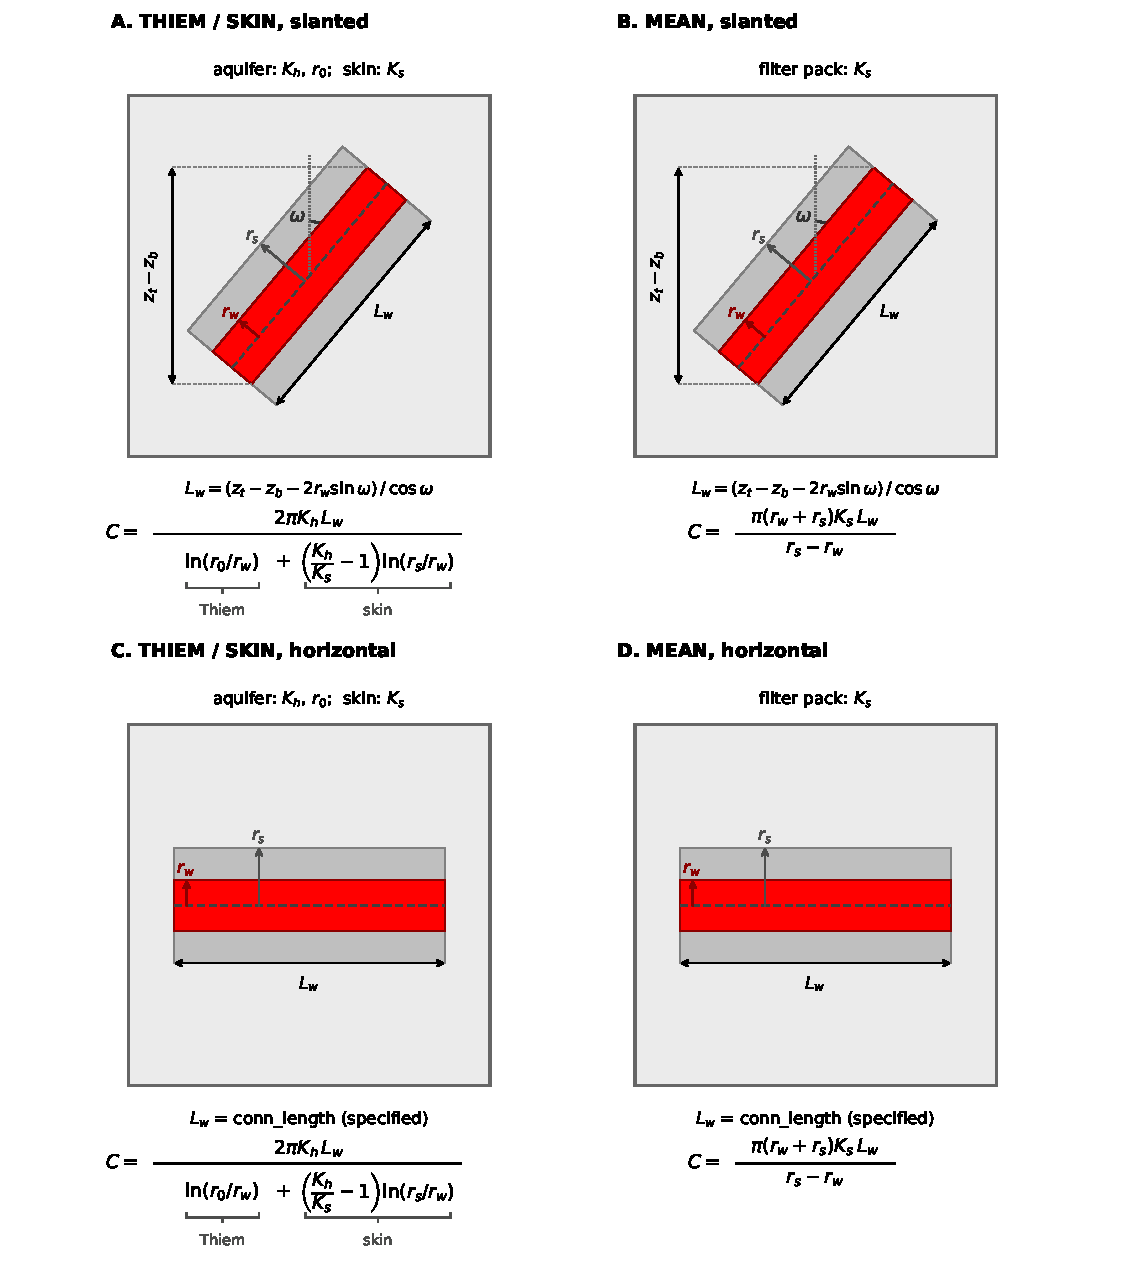
\includegraphics[width=0.78\textwidth]{./Figures/MAWNonVerticalConcept.pdf}
	\caption[Conceptual diagram of the in-cell screen length and conductance for non-vertical connections]{Conceptual diagram showing how the in-cell screen length $L_w$ and the saturated conductance are calculated for non-vertical multi-aquifer well connections. The red rectangle is the well screen (radius $r_w$) and the gray rectangle is the surrounding filter pack (radius $r_s$). For a slanted connection (A, B) the in-cell screen length is derived from the vertical screen extent $z_t - z_b$, the well radius, and the tilt angle $\omega$; for a horizontal connection (C, D) the in-cell screen length is specified directly as the connection length. The \texttt{THIEM}, \texttt{SKIN}, and \texttt{CUMULATIVE} equations (A, C) use the radial flow geometry in the horizontal plane (aquifer hydraulic conductivity $K_h$ and effective radius $r_0$), and the Thiem and skin terms of the denominator are identified by underbraces; the \texttt{MEAN} equation (B, D) uses the cylindrical flow through the filter pack between the well radius $r_w$ and skin radius $r_s$}
	\label{fig:mawnvconcept}
	\end{center}
\end{figure}

\subsection{Horizontal Connections and Radial Collector Wells}

The \texttt{THIEM}, \texttt{SKIN}, and \texttt{CUMULATIVE} conductance equations use the radial flow geometry in the horizontal plane (the horizontal hydraulic conductivities $K_{11}$ and $K_{22}$ and a horizontal effective radius). Applying the length correction to these equations for a strongly deviated or horizontal connection therefore yields only an approximate conductance, because the radial flow to a horizontal screen occurs in a vertical plane that involves the vertical hydraulic conductivity. \cite{halford2002} and \cite{konikow2009} note that suitable cell-to-well conductance equations for horizontal wells are not well defined. The \texttt{MEAN} conductance equation does not depend on the cell flow geometry and is recommended for horizontal connections. The \mf~program issues a warning when a near-horizontal connection uses a radial conductance equation.

For a horizontal connection that uses the \texttt{MEAN} conductance equation, the screen top and bottom ($\mli{TOPSCRN}_n$ and $\mli{BOTSCRN}_n$) do not affect the magnitude of the saturated conductance, because the vertical screen extent cancels with the length-correction factor (eq.~\ref{eqn:mawnv-lcorr}) and the conductance depends only on the specified connection length. The screen top and bottom do, however, determine the elevation range over which the connection saturates and dewaters as the water table passes through the borehole (the saturation is calculated from $\mli{TOPSCRN}_n$ and $\mli{BOTSCRN}_n$). The screen top and bottom should therefore be set to the top and bottom of the horizontal borehole; that is, for a horizontal connection whose axis is at elevation $z_0$, $\mli{TOPSCRN}_n = z_0 + r_w$ and $\mli{BOTSCRN}_n = z_0 - r_w$, so that the vertical screen extent equals the well diameter, $2 r_w$. The \mf~program snaps $\mli{TOPSCRN}_n$ to $\mli{BOTSCRN}_n + 2 r_w$ when the specified extent is essentially equal to the well diameter and otherwise issues a warning.

A radial collector well (also called a Ranney well) is a common application of horizontal connections. A radial collector well consists of a central caisson with several horizontal laterals that radiate outward near the base of an aquifer. Such a well can be represented as a single multi-aquifer well with one connection to each cell traversed by a lateral. Each lateral connection is specified with a tilt angle of $90^{\circ}$ and a connection length equal to the length of the lateral within the connected cell, and the \texttt{MEAN} conductance equation is used so that the calculated conductance is exact for the horizontal laterals. An example radial collector well is shown in figure~\ref{fig:mawcollector}. The well is represented as a single multi-aquifer well with 49 connections to the GWF model: one vertical connection to the central caisson cell and 48 horizontal lateral connections, with 12 cells in each of the four lateral directions.

\begin{figure}[!ht]
	\begin{center}
	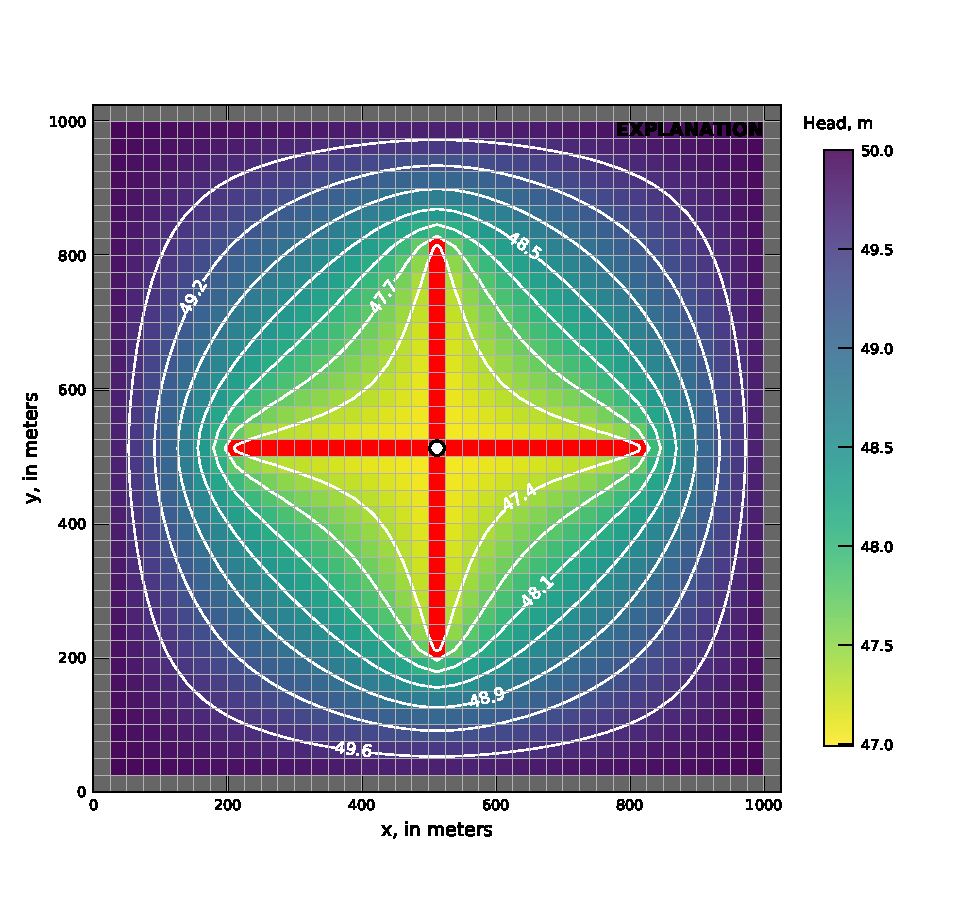
\includegraphics[width=0.55\textwidth]{./Figures/MAWNonVerticalCollector.pdf}
	\caption[Map showing the configuration and simulated heads for an example radial collector well]{Map showing the configuration and simulated heads for an example radial collector (Ranney) well simulated with the Multi-Aquifer Well (MAW) Package. The well is represented as a single multi-aquifer well with a vertical caisson connection (open circle) and four horizontal laterals (red cells) specified as non-vertical connections with a tilt angle of $90^{\circ}$. Constant-head cells (gray) surround the active model domain. The simulated head field and contours show the drawdown that develops along the laterals in response to pumping from the well}
	\label{fig:mawcollector}
	\end{center}
\end{figure}

The effect of the length correction on the simulated well head is illustrated by a transient simulation of the example radial collector well in which the well is pumped and then allowed to recover (fig.~\ref{fig:mawcollectorts}). When the horizontal laterals are represented as non-vertical connections, the in-cell screen length used to calculate the saturated conductance is the length of the lateral within each cell, which produces a large saturated conductance and a modest drawdown in the well. When the same lateral cells are instead connected with thin vertical screens (that is, the length correction is not applied), the much smaller saturated conductance produces substantially more drawdown in the well for the same pumping rate, illustrating the importance of using the in-cell screen length to calculate the saturated conductance for non-vertical connections.

\begin{figure}[!ht]
	\begin{center}
	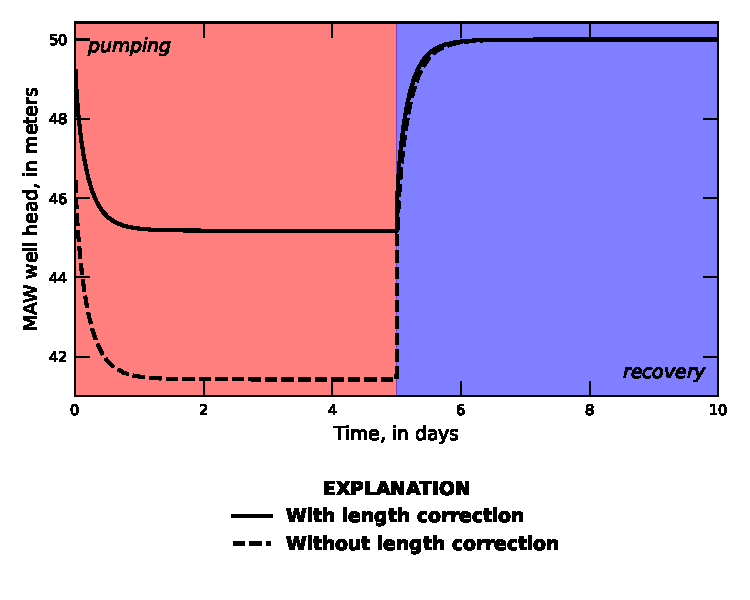
\includegraphics[width=0.5\textwidth]{./Figures/MAWNonVerticalTimeseries.pdf}
	\caption[Simulated well head for the example radial collector well]{Simulated multi-aquifer well head for a transient simulation of the example radial collector well shown in figure~\ref{fig:mawcollector}. The well head is shown for the laterals represented as horizontal connections (with the length correction) and as thin vertical screens (without the length correction). The pumping and recovery periods are shaded red and blue, respectively}
	\label{fig:mawcollectorts}
	\end{center}
\end{figure}

\subsection{Usage Considerations}

Each multi-aquifer well connection represents the exchange between the well and a single GWF cell. The tilt angle and connection length scale the saturated conductance for that connection only; they do not route flow through intervening cells. A well that physically passes through more than one cell---such as a slanted well or a horizontal lateral---must therefore have a separate connection, with its own connection length, to each cell that it penetrates, as in the radial collector well example (fig.~\ref{fig:mawcollector}). For the \texttt{THIEM}, \texttt{SKIN}, and \texttt{CUMULATIVE} conductance equations, only one connection can be specified per cell; the \texttt{MEAN} conductance equation allows more than one connection to the same cell.

For a partially saturated cell, the connection saturation is calculated from the vertical screen extent ($\mli{TOPSCRN}_n$ and $\mli{BOTSCRN}_n$); the saturated conductance described above is multiplied by this saturation. For a slanted connection the vertical screen extent is the vertical projection of the screen, and for a horizontal connection it is the borehole diameter, as discussed above.

The length correction requires only the screen elevations, well radius, and tilt angle---it does not require the horizontal cell dimensions or the vertical hydraulic conductivity---so non-vertical connections are supported for all grid types (DIS, DISV, and DISU).
